\documentclass{beamer}
%\documentclass[handout]{beamer}
\usetheme{Antibes}

\usepackage{fontspec}
\usepackage[catalan]{babel}
\usepackage{hyperref}
\usepackage[normalem]{ulem}

\AtBeginSection[]
{
	\begin{frame}
		\frametitle{Contingut}
		\tableofcontents[currentsection]
	\end{frame}
}

\AtBeginSubsection[]
{
	\begin{frame}
		\frametitle{Contingut}
		\tableofcontents[currentsection,currentsubsection]
	\end{frame}
}

\title{Construcció d'una orquestra amb Raspberry Pi}
\author{Arnau Canyadell Miquel \and Joan Marcè Igual}

\begin{document}

\frame{\titlepage}
\section{Introducció}

\begin{frame}
	\frametitle{Descripció del projecte}
	Crear amb Raspberry Pi una orquestra musical formada per un director i uns quants músics que interpreten el que els mana el director.
	\begin{figure}
		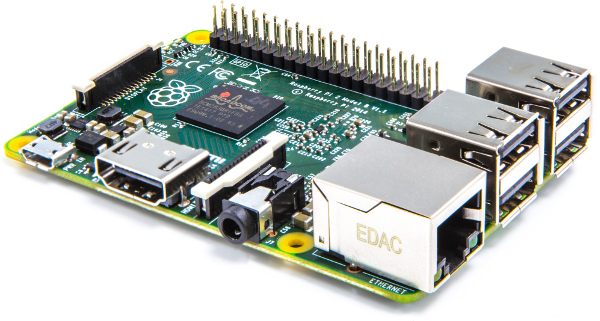
\includegraphics[width=0.475\linewidth]{images/raspberry}
		\hfill
		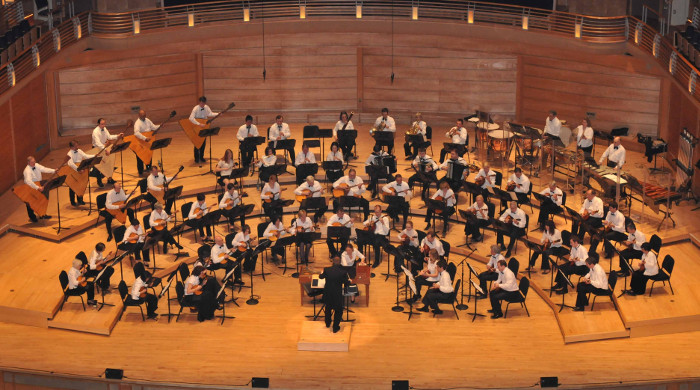
\includegraphics[width=0.475\linewidth]{images/orchestra}
	\end{figure}
\end{frame}

\section{Feina feta}
\begin{frame}
	\frametitle{Què hem fet fins ara?}
	\begin{itemize}[<+->]
		\item Establiment dels objectius
		\item Analitzat el codi del director
		\item Programat el codi de l'intèrpret (músic)
		\item Codi per configurar una raspberry pi qualsevol per a funcionar com a músic
		\item Canvis en el codi del director
	\end{itemize}
\end{frame}

\begin{frame}
	\frametitle{Principals problemes trobats}
	\begin{itemize}[<+->]
		\item Mida de les targetes SD. 4 GB no era suficient.
		\item Àudio en la raspberry pi. No hem sabut canviar el dispositiu de sortida des de l'entorn de comandes. Hem hagut d'instal·lar l'entorn gràfic a la raspberry pi.
	\end{itemize}
\end{frame}

\section{Objectius}
\begin{frame}
	\frametitle{Feina a fer a partir d'ara}
	\begin{itemize}[<+->]
		\item Bot de Telegram que reprodueixi midi
	\end{itemize}
	\begin{figure}
		\hfill
		
\includegraphics[width=0.2\textwidth]{images/telegram}
		\hfill
		
\includegraphics[width=0.475\textwidth]{images/mobile}
		\hfill
	\end{figure}
\end{frame}

\section{Demo}
\begin{frame}
	\frametitle{Demo en directe}
	\begin{figure}
		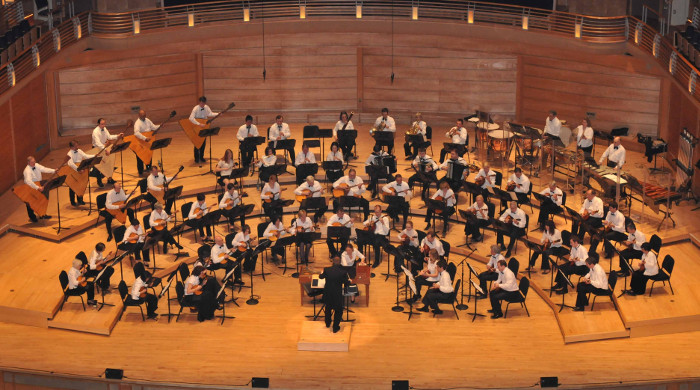
\includegraphics[width=\linewidth]{images/orchestra}
	\end{figure}
\end{frame}

\end{document}